
{\sl This fieldstone was developed in collaboration with Job Mos}.
\index{contributors}{J. Mos}

This benchmark is taken from \cite{dohu03} and is described fully in section \ref{mms}. 
In order to illustrate the behavior of selected mixed finite elements in the solution 
of stationary Stokes flow,  we consider a two-dimensional problem 
in the square domain $\Omega=[0,1]\times[0,1]$, which possesses a closed-form analytical 
solution. The problem consists of determining the velocity field ${\bm v} = (u,v)$ and the 
pressure $p$ such that 
\[
\eta \Delta \vec{v} - \vec{\nabla} p + \vec{b} = \vec{0}   \quad\quad {\rm in} \; \Omega
\]
\[
\vec{\nabla} \cdot \vec{v} = 0 \quad\quad {\rm in} \; \Omega
\]
\[
\vec{\bm v}=\vec{0} \quad\quad {\rm on} \; \Gamma_D
\]
where the fluid viscosity is taken as $\eta=1$. 


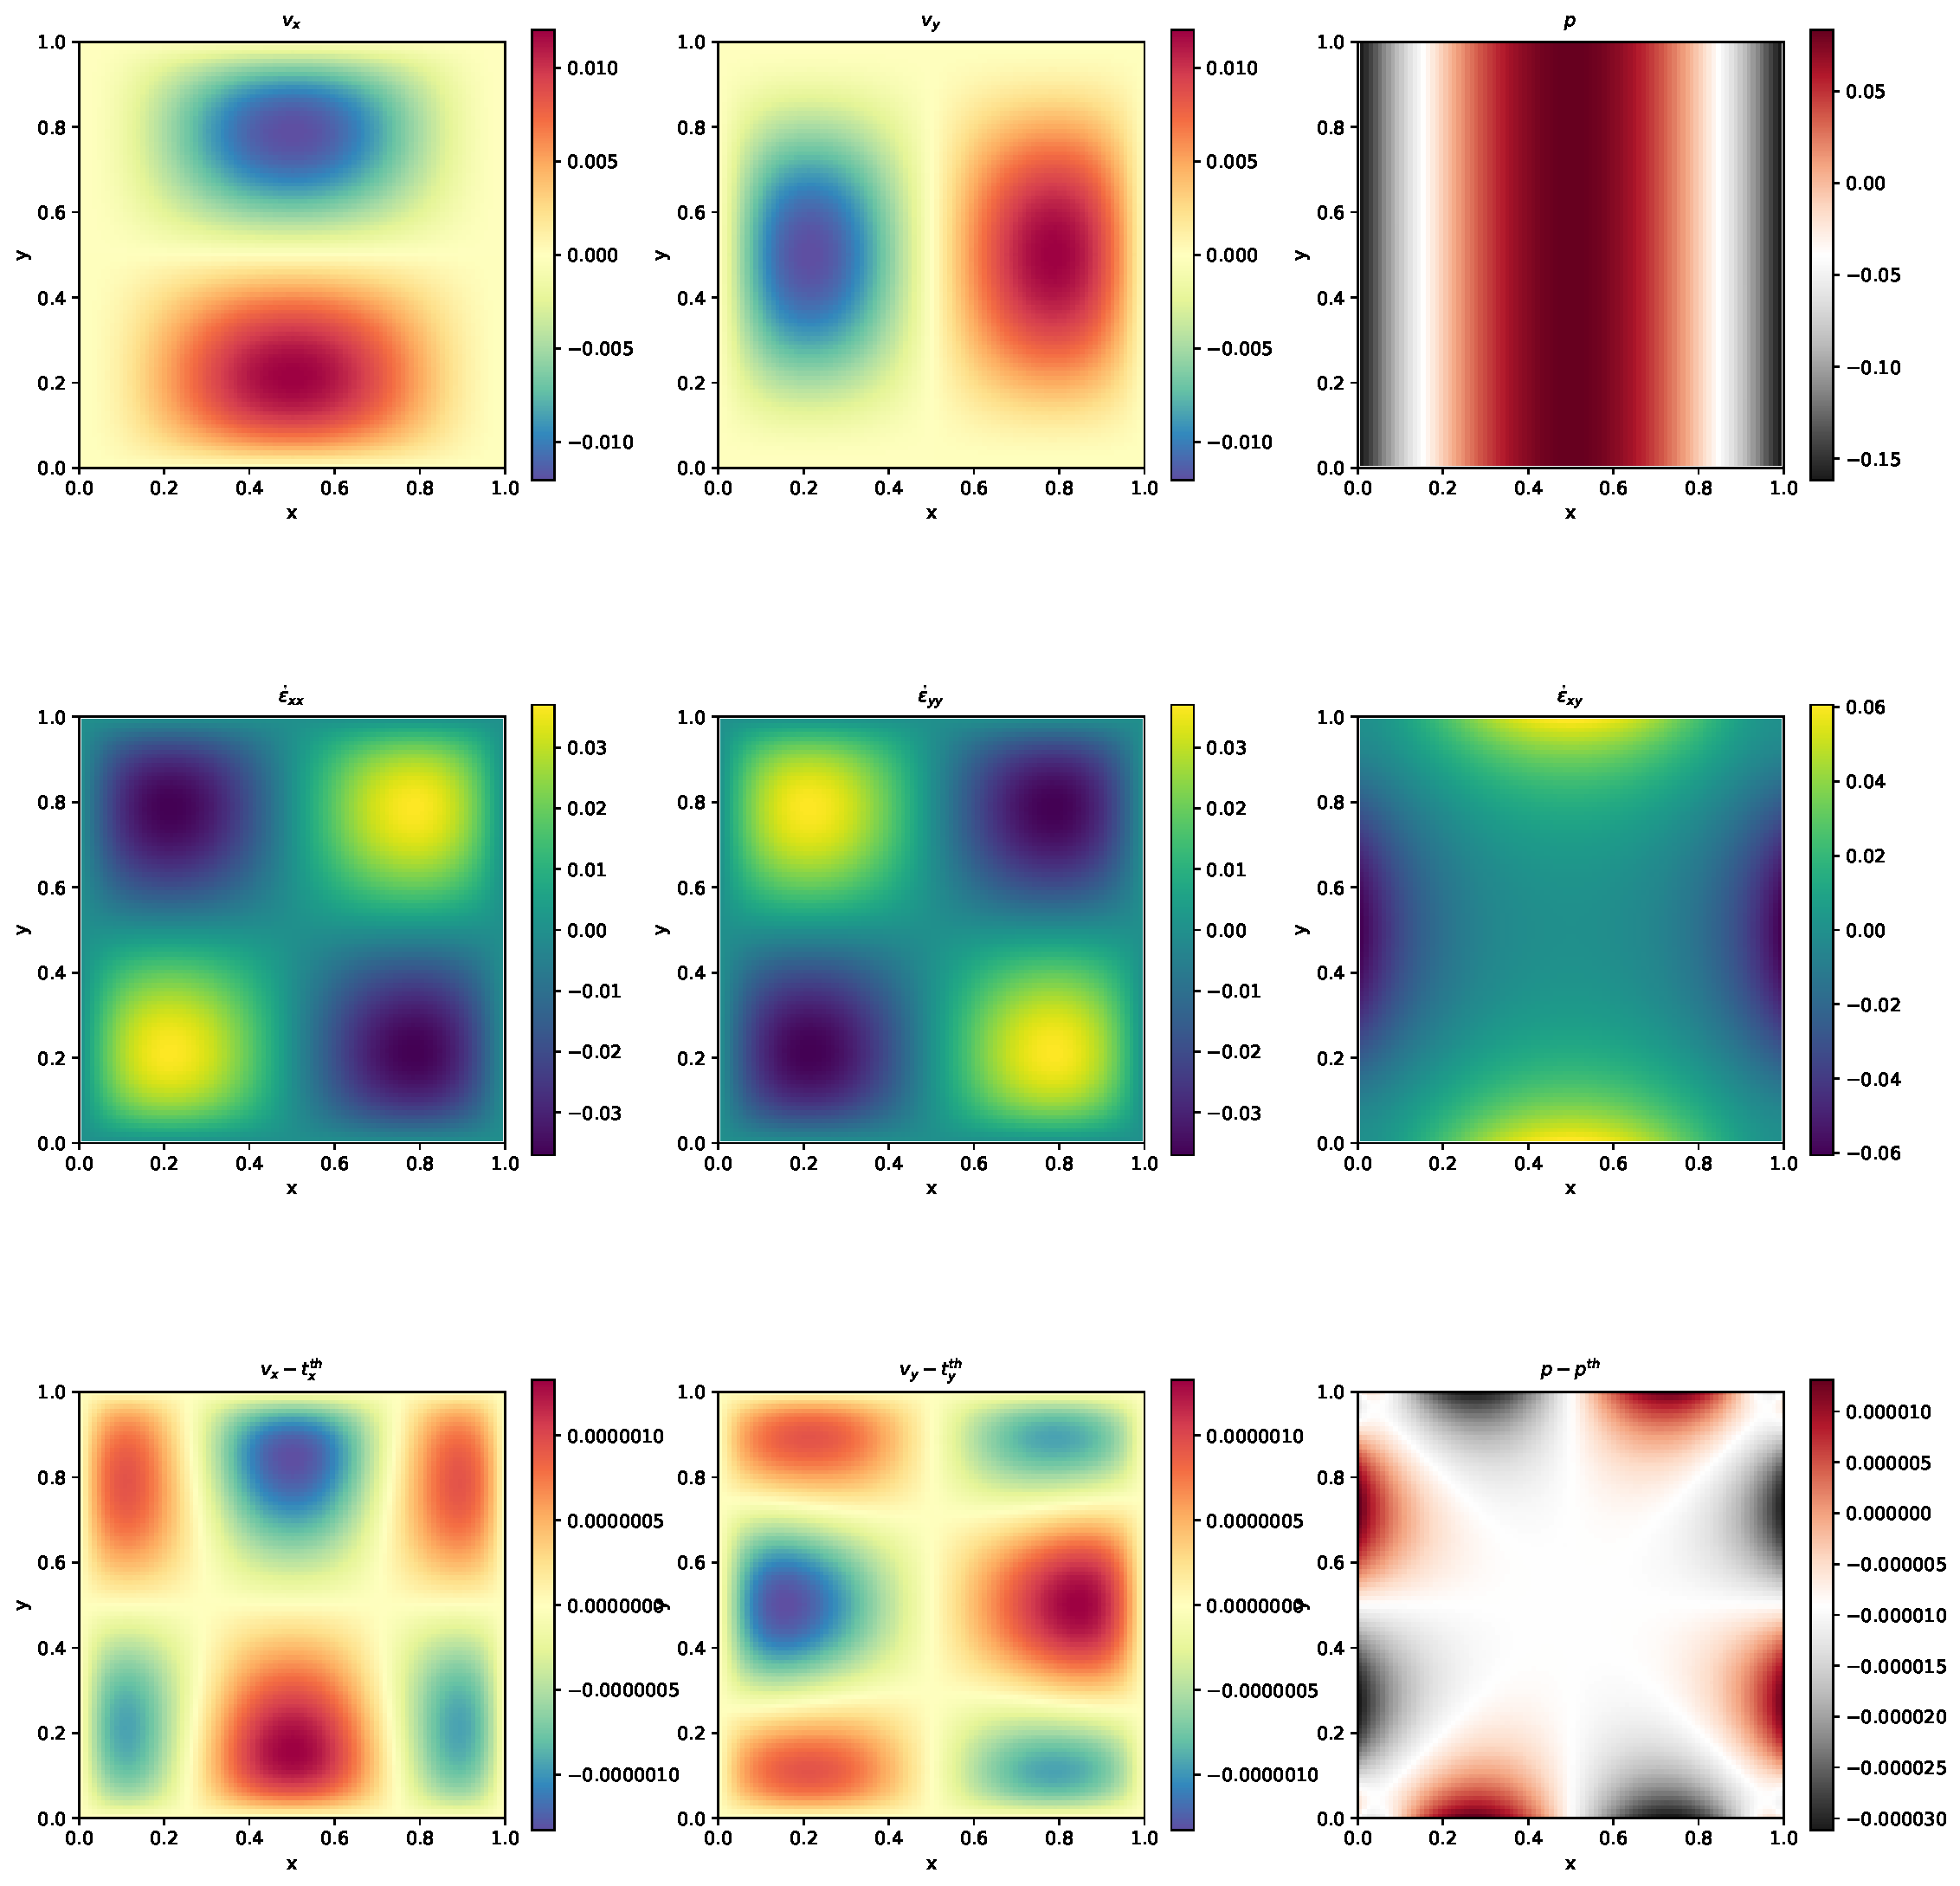
\includegraphics[width=16cm]{python_codes/fieldstone_01/solution.pdf}

\begin{center}
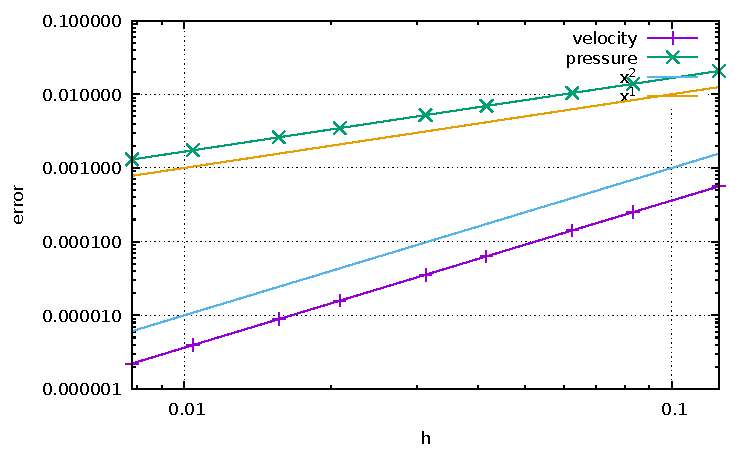
\includegraphics[width=12cm]{python_codes/fieldstone_01/errors.pdf}\\
Quadratic convergence for velocity error, 
linear convergence for pressure error, as expected.
\end{center}

\index{stones}{$Q_1\times P_0$ element}
\index{stones}{Penalty Formulation} 
\index{stones}{Analytical Solution}
